% -*- TeX:de -*-
\NeedsTeXFormat{LaTeX2e}
\documentclass[12pt,a4paper]{article}
\usepackage[german]{babel} % german text
\usepackage[DIV12]{typearea} % size of printable area
\usepackage[T1]{fontenc} % font encoding
%\usepackage[latin1]{inputenc} % most likely on Windows
\usepackage[utf8]{inputenc} % probably on Linux
\usepackage{multicol}

% PLOTTING
\usepackage{pgfplots} 
\usepackage{pgfplotstable}
\usepackage{url}
\usepackage{graphicx} % to include images
\usepackage{tikz}
\usepackage{subfigure} % for creating subfigures
\usepackage{amsmath} % a bunch of symbols
\usepackage{amssymb} % even more symbols
\usepackage{booktabs} % pretty tables
\usepackage{makecell} % multi row table heading

% a floating environment for circuits
\usepackage{float}
\usepackage{caption}

%\newfloat{circuit}{tbph}{circuits}
%\floatname{circuit}{Schaltplan}

% a floating environment for diagrams
%\newfloat{diagram}{tbph}{diagrams}
%\floatname{diagram}{Diagramm}

\selectlanguage{german} % use german

\begin{document}

%%%%%%% DECKBLATT %%%%%%%
\thispagestyle{empty}
			\begin{center}
			\Large{Fakultät für Physik}\\
			\end{center}
\begin{verbatim}


\end{verbatim}
							%Eintrag des Wintersemesters
			\begin{center}
			\textbf{\LARGE SS 14}
			\end{center}
\begin{verbatim}


\end{verbatim}
			\begin{center}
			\textbf{\LARGE{Physikalisches Praktikum\\ für das Bachelorstudium}}
			\end{center}
\begin{verbatim}




\end{verbatim}

			\begin{center}
			\textbf{\LARGE{PROTOKOLL}}
			\end{center}
			
\begin{verbatim}

\end{verbatim}

			\begin{flushleft}
			\textbf{\Large{Experiment (Nr., Titel): PS9 - Heißluftmotor - Stirlingprozess}}\\
							%Experiment Nr. und Titel statt den Punkten eintragen
			\LARGE{PS09 }	
			\end{flushleft}

\begin{verbatim}

\end{verbatim}	
							%Eintragen des Abgabedatums, oder des Erstelldatums des Protokolls
			\begin{flushleft}
			\textbf{\Large{Datum:}} \Large{10.04.2014}
			\end{flushleft}
			
\begin{verbatim}
\end{verbatim}
							%Namen der Protokollschreiber
		\begin{flushleft}
			\textbf{\Large{Namen:}} \Large{Patrick Braun, Johannes Kurz}
			\end{flushleft}

\begin{verbatim}


\end{verbatim}
							%Kurstag und Gruppennummer, zb. Fr/5
			\begin{flushleft}
			\textbf{\Large{Kurstag/Gruppe:}} \Large{DO/4}
			\end{flushleft}

\begin{verbatim}

\end{verbatim}
							%Name des Betreuers, das Praktikum betreute.
			\begin{flushleft}
			\LARGE{\textbf{Betreuer:}}	\Large{Johanna Akbarzadeh}	
			\end{flushleft}

%%%%%%% DECKBLATT ENDE %%%%%%%
\pagebreak
\setlength{\columnsep}{20pt}
\begin{multicols}{2}

%%%%%%%%%%%%%%%%%%%%%%%%%%%%%%%%%%%%%%%%%%%%%%%%

%\begin{figure}[H]
%	\centering
%	\includegraphics[scale=0.35]{./data/beugung.png}
%	\caption{Beugungsmuster Einzelspalt (echtes Foto; schwarz durch weiß ersetzt)}
%	\label{fig:beugungsmuster}
%\end{figure}


%\begin{figure}[H]
%	\centering
%	\pgfplotstabletypeset[
%			columns={abstand, n},
%			col sep=&,
%			columns/abstand/.style={precision=2, zerofill, column name=\makecell{$Abstand$\\$(\pm 0.05)[mm]$} }, 
%			columns/n/.style={column name=\makecell{$n$\\$(Ordnung)$}, precision=0},
%			every head row/.style={before row=\hline,after row=\hline\hline},
%			every last row/.style={after row=\hline},
%			every first column/.style={column type/.add={|}{} },
%			every last column/.style={column type/.add={}{|} }
%			]{
%			abstand & n
%			12.9 & 1
%			24.45 & 2
%			37.40 & 3
%			49.35& 4
%			62.45 & 5
%			74.45 & 6
%			87.45 & 7
%			100.25 & 8
%			
%			}
%	\caption{Messwerte Einzelspalt}
%	\label{tab:werte_einzelspalt}
%\end{figure}


%%%%%%%%%%%%%%%%%%%%%%%%%%%%%%%%%%%%%%%%%%%%%%%%
%%%%%%%%%%%%%%%%%%%%%%%%%%%%%%%%%%%%%%%%%%%%%%%%
\noindent Im Folgenden werden unterschiedliche Anwendungen einer Stirling-Maschine untersucht. Als Wärmekraftmaschine auf Grundlage des Carnotprozesses und in abgeänderter Form als Kältemaschine.\\
Als wichtigstes Maß eines Motors errechnen wir den Wirkungsgrad jeder Anwendung.


\section{Der Heißluftmotor als Wärmekraftmaschine}
In diesem Teil des Experiments bestimmen wir den Wirkungsgrad eines Stirlingmotors über die Leistung welche zugeführt wird und abgenommen werden kann. Zu erst bestimmen wir den idealen Wirkungsgrad, danach den realen Wirkungsgrad und zu Letzt den Wirkungsgrad des Motors.

\subsection{Grundlagen}
Für die Berechnungen benötigen wir folgende Formeln ([1] (pp. 6-8)):\\
$$\eta{ideal} = \frac{T_1 - T_2}{T_1}$$
Bei diesem idealen Verhalten geht keine Energie über Reibung oder Abstrahlung verloren.
$$\eta_{real} = \frac{P_{Motor}}{P_{Zugeführt}}$$
Der reale Wirkungsgrad ist der aussagekräftigste. Dabei wird die aufgewendete Leistung der abnehmbaren Leistung gegenüber gestellt.
$$\eta_{Motor} = \frac{P_{Motor}}{\oint p dV * f}$$
Den Wirkungsgrad des Motors erhalten wir durch die Leistung des Motors (jeweilig beschrieben durch Abnehmer) gebrochen durch die Leistung beschrieben durch die eingeschlossene Fläche im Carnotprozess (entspricht der Energie) mal die Frequenz. 
\\
Im realen Prozess ergibt sich aber keine schön abgegrenzte Fläche wie in [1] dargestellt sondern eine wie in Abbildung \ref{fig:real_carnot}.

\begin{figure}[H]
	\centering
	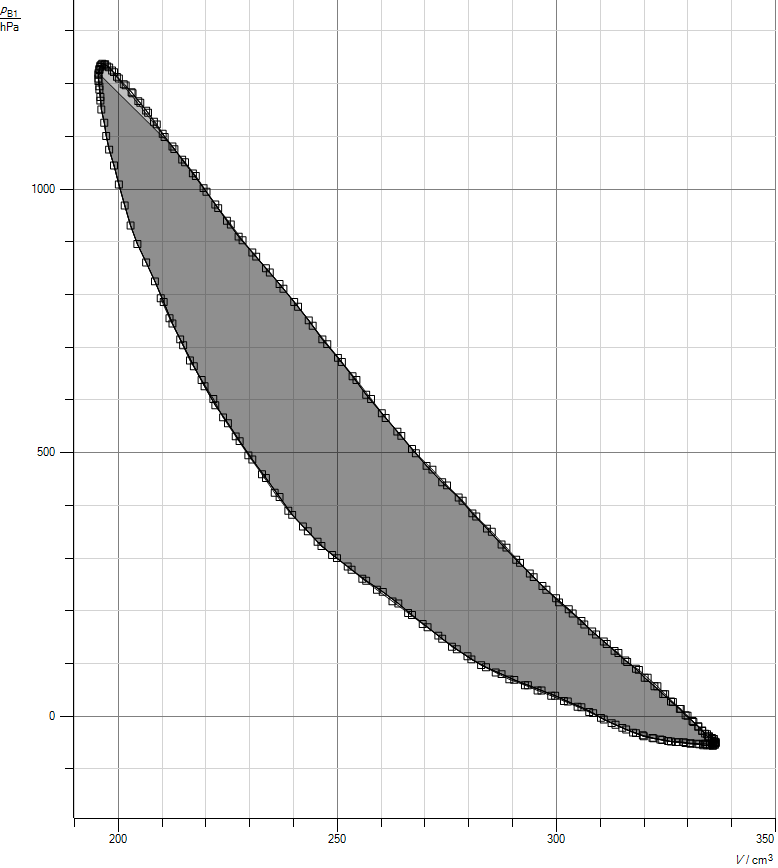
\includegraphics[scale=0.25]{./data/kennlinie_stirling_ohnelast.png}
	\caption{Kennlinie im pV-Diagramm eines realen Prozesses im Leerlauf}
	\label{fig:real_carnot}
\end{figure}

\subsection{Versuchsaufbau}
In diesem Experiment wird ein bereits aufgebauter Stirlingmotor mit einer Heizspindel und einer Kühlung betrieben (Abbildung  \ref{fig:stirlingMotor_3D}). Als Grundlage dient der bereits beschriebene Carnotprozess. Druck und Volumen werden mit Cassy-Lab erfasst. Kühlung und Heizung können über Netzteile gesteuert werden. Die Frequenz wird über ein magnetisches Rad mit Löchern und einem Stroboskop gemessen.\\
\\
Das Volumen des Zylinder ergibt sich durch (auf den Nullpunkt angepasst):\\
$Volumen = Weg (\pm 0.08mm) * Fläche (28.3 \pm 0.1)mm + 195 = $\\ %%%% TODO ergebnis %%%%%
Der Bereich für den Druck\\
$Druck (-2000 - +2000 \pm 2) hPa$\\

\begin{figure}[H]
	\centering
	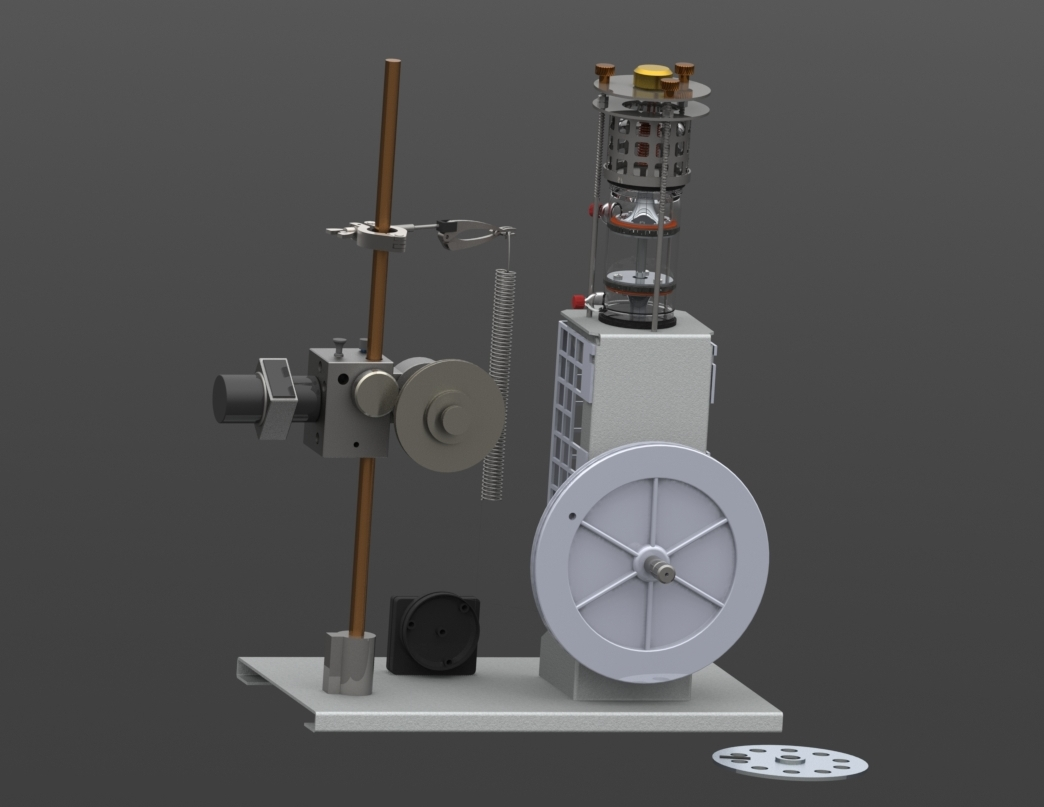
\includegraphics[scale=0.20]{./data/3D-Model/PS9-model_neutral01.JPG}
	\caption{Versuchsaufbau als 3D Modell}
	\label{fig:stirlingMotor_3D}
\end{figure}

\subsection{Resultate}
\textbf{1. Leerlaufbetrieb:}\\
Leerlaufkreisfrequenz:\\
$\omega=(50.0 \pm 1.3)s^{-1}$
$$\eta_{ideal}=(54.6 \pm 2.8)\%$$
\textbf{2. Unbelastet:}\\
Heizleistung:\\
Strom: $(20 \pm 1) A$\\
Spannung: $(14 \pm 0.5) V$\\
$P_{Heizung}=(280 \pm 18)W$\\
$$\eta_{real}=(10.65 \pm 0.71)\%$$\\

%
%$A_1 = 37130 hPa*cm^3$\\
%$A_2 = 38140 hPa*cm^3$\\
%$f_2 = \frac{25.32}{3} Hz$\\
%$A_3 = 37530 hPa *cm^3$\\
%$f_3 = \frac{37.82}{5} Hz$\\
%$A_4 = 36660 hPa * cm^3$\\
%$f_4 = \frac{25.28}{3} Hz$\\
%$A_5 = 37000 hPa * cm^3$\\
%$f_5 = \frac{76.18}{10}$\\
%
%
%
%$A_6 = 38720  hPa * cm^3$\\
%$A_7 = 37250  hPa * cm^3$\\
%$f_{6-1} = 7.77 Hz$\\
%$f_{6-2 / 7} = 15.49 / 2 Hz$\\



\noindent \textbf{3. Belastet:}\\
$r = (25.0 \pm 0.2)cm$\\
$F_1 = (1.00 \pm 0.05)N$\\
$f_1 = (5.4 \pm 0.05)Hz$\\
$\eta_{motor1}=(3.03\pm 0.25)\%$\\
$F_2=(0.97\pm 0.05)N$\\
$f_2 = (5.5 \pm 0.05)Hz$\\
$\eta_{motor2}=(2.99\pm 0.25)\%$\\
$$\eta_{motor}=(3.01\pm 0.25)\%$$


\subsection{Diskussion}

Die Unterschiede zwischen idealem und realem Wirkungsgrad, sowie demjenigen unter Belastung sind deutlich zu erkennen:\\
$\eta_{ideal}=(54.6 \pm 2.8)\%$\\
$\eta_{real}=(10.65 \pm 0.71)\%$\\
$\eta_{motor}=(3.01\pm 0.25)\%$\\

\noindent Die Verluste durchReibung, Konvektion und Wärmestrahlung sowie die unrealistische Annahme eines vollständig reversiblen Prozesses führen zu einem etwa 5mal niedrigeren realem Wirkungsgrad im Leerlauf, im Vergleich zur Theorie.\\
Die Reibungsverluste bei Belastung, also die eines Motors, der effektiv Arbeit an einer Vorrichtung verrichtet, reduzieren den Wirkungsgrad nochmals um 1/3.\\

\noindent Der vergleichsweise große Unsicherheitsbereich von $\eta_{ideal}$ entsteht dabei durch eine größere Fehlerabschätzung bei Druck und Volumen, als das Messvermögen der CASSY-Sensoren verlangen würde. Da jedoch der aufgezeichnete Kreisprozess nicht komplett stabil (im Rahmen der Auflösung) läuft, haben wir uns für einen etwas gröberen Bereich entschieden.\\

\noindent Die Messergebnisse zeigen das erwartete Verhalten und demonstrieren eindrucksvoll die schwache Umsetzung des Stirling-Motors von Energie in nutzbare Arbeit.\\
Sicherlich gäbe es jedoch einiges Verbesserungsmöglichkeiten; Auch ohne den Motor fundamental umzubauen, ließen sich vor allem die beweglichen Teile sicherlich noch besser lagern um Reibungsverluste zu minimieren.\\
Andere Materialien im Bereich, in dem Temperaturaustausch stattfindet könnten hier zu besseren Ergebnissen führen.\\
Ein Getriebe oder auch ein optimiertes Schwungrad könnten zumindest den Wirkungsgrad im Vollbetrieb verbessern.\\
Große Verbesserungen sind jedoch nicht zu erwarten.\\

\noindent Die Messung der Frequenz mit Stroboskop und Lochscheibe scheint, abgesehen von komplizierteren Sensor-Messaufbauten, die beste Lösung für schnelle und genaue Ergebnisse zu sein. Auch wenn völliger Stillstand der wahrgenommenen Löcher nicht zu erreichen war, sind die Ergebnisse jedoch mehr als genau genug im Vergleich zu den Schwankungen des Motors selbst.\\
Der reale Wirkungsgrad wurde aus einem Mittel aus 6 Einzelmessungen (pV-Diagramm sowie Frequenz) im Abstand von etwa 1min bestimmt. Die Unterschiede zwischen den einzelnen Messungen sind dabei deutlich größer, als die Messunsicherheit der Stroboskop-Methode.\\
Auch die Messung mit dem Bremszaum ist im Vergleich zu den Schwankungen des Motors selbst, ausreichend genau (ideale $90^\circ$ zwischen Bremszaum und Federwaage sind natürlich nicht gegeben, der Winkel bleibt jedoch gut stabil und die Abweichung des Winkels hat nur kleine Auswirkungen auf das Ergebnis).



%%%%%%%%%%%%%%%%%%%%%%%%%%%%%%%%%%%%%%%%%%%%%%%%
%%%%%%%%%%%%%%%%%%%%%%%%%%%%%%%%%%%%%%%%%%%%%%%%
\section{Die Stirling-Maschine als Kältemaschine}

\subsection{Grundlagen}


\subsection{Resultate}


Kühlraumtemperatur:\\ 
$T= (5.6 \pm 0.5)^{\circ}C$\\
\indent (deutliche Schwankungen)\\
Zugeführte Leistung:\\
$P=(82.8 \pm 4.6)W$\\
%$230V * (0.36 \pm 0.03) A$\\
\noindent Kühlung (= Heizleistung der Heizwendel):\\ 
$U= (8.3 \pm 0.7)V$\\
$A_{unten} = (1.7 \pm 0.2)A$\\
%$U_{oben} = (8.5 \pm 0.5)V$\\
%$A_{oben} = (1.8 \pm 0.1)A$\\
\noindent Umdrehungsfrequenz:\\
$f = (5.06\pm 0.05)Hz$\\
Wirkungsgrad:\\
$$\eta_{Kaelte}=(17.04\pm 2.7)\%$$

\subsection{Diskussion}





\section{Quellen}
$[1]$ Anleitung, \url{http://www.univie.ac.at/anfpra/neu1/ps/ps9/PS9.pdf}\\

\end{multicols}

\begin{figure}[H]
	\centering
	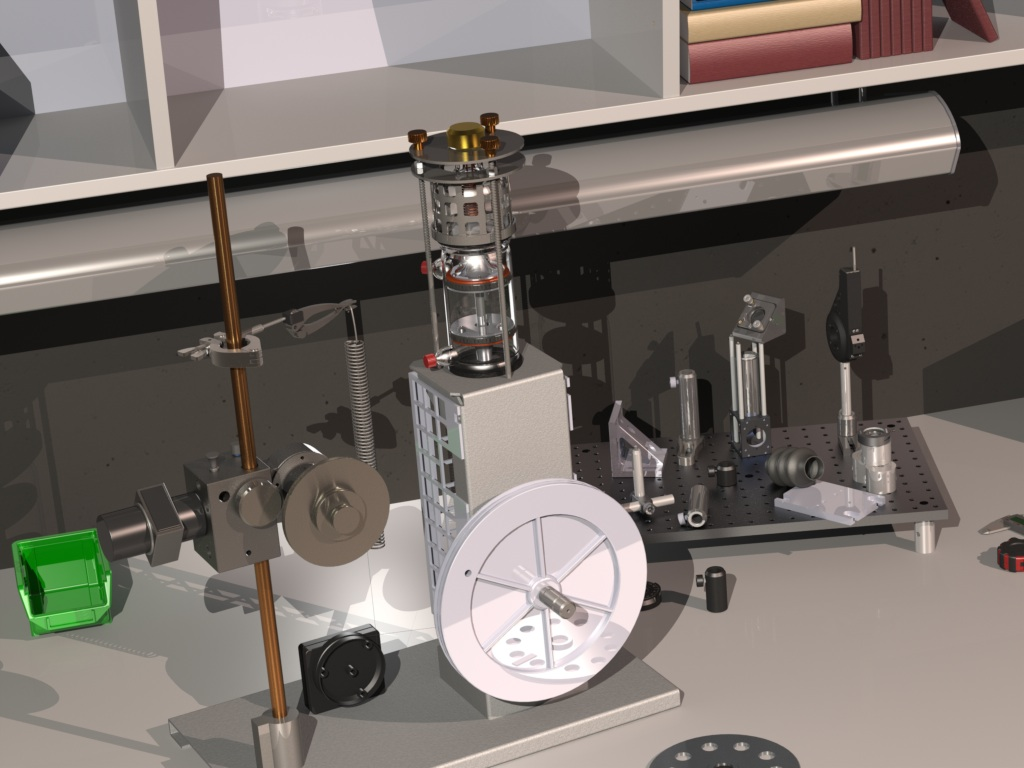
\includegraphics[scale=2]{./data/3D-Model/PS9-model_desk01.JPG}
	%\caption{}
	\label{fig:stirlingMotor_3D-desktop}
\end{figure}

\end{document}